\section{Problema 1: Roban\'umeros}

\subsection{Presentaci\'on del problema}
El Roban\'umeros es un juego de cartas para dos jugadores. Al iniciar se dispone sobre la mesa una secuencia
de cartas boca arriba. Cada carta tiene dibujado un n\'umero entero (no necesariamente positivo). El
Roban\'umeros se juega por turnos, alternando un turno para cada jugador. En su turno el jugador debe
elegir uno de los dos extremos (izquierdo o derecho) de la secuencia que actualmente est\'aen la mesa y
robar cartas comenzando por dicho extremo. Puede robar la cantidad de cartas que quiera pero tiene que
robar cartas adyacentes a partir del extremo elegido. Por ejemplo, si las cartas en la mesa son

$$ 2, ~ -4, ~ 6, ~ 1, ~ 9, ~ -10 $$

Entonces el jugador podr\'ia robar las cartas $2, ~ -4, ~ 6$ empezando por la izquierda por ejemplo o bien
las cartas $-10, ~ 9, ~ 1, ~ 6$ empezando desde la derecha, pero no podr\'ia robar las cartas $2, ~ 6, ~ 1$
ya que se estar\'ia salteando la carta $-4$. Tampoco ser\'ia posible robar las cartas $6, ~ 1, ~ 9$ ya que si
bien son adyacentes, la secuencia no se inicia en alguno de los extremos.


En su turno, el jugador debe robar al menos una carta y el juego termina cuando ya no quedan cartas
en la mesa. En este momento, cada jugador suma los valores de las cartas que rob\'o y el que obtenga una
suma mayor gana el juego.

Mingo y An\'ibal son dos jugadores expertos de Roban\'umeros y nos retaron a escribir un algoritmo que
juegue tan bien como ellos. Es decir, tenemos que escribir un algoritmo que juegue en forma \'optima a
este juego suponiendo que su contrincante es tan inteligente como \'el. El programa a implementar debe
tomar una secuencia inicial de cartas y debe indicar qu\'e cartas robar\'ia Mingo y An\'ibal en cada turno,
asumiendo que ambos juegan de manera \'optima a este juego. En este contexto, decimos que un jugador
juega de manera \'optima si la diferencia de puntos obtenida a su favor es la mayor diferencia que se puede
obtener frente a un oponente que juega tambi\'en de manera \'optima cada situaci\'on que se le deje. En caso
de haber m\'as de una soluci\'on \'optima, el algoritmo puede devolver cualquiera de ellas. Se pide que el
algoritmo desarrollado tenga una complejidad temporal de peor caso de $O(n^3)$, donde $n$ es la cantidad
de cartas en la secuancia inicial.

\subsection{Resoluci\'on}

Defino la funcion $f(i,j)$ como la solucion \'optima usando de las cartas $i$ a $j$. Esto es, lo m\'aximo que puedo agarrar con las cartas de la izquierda (1*) o de la derecha (2*). 

\begin{enumerate}
\item[(1*)] \label{x_izq} Supongamos que por la izquierda lo mejor que puedo hacer es usando las primeras $k$ cartas. Significa que el valor que puedo tomar es $\sum_{t=i}^{k} carta[t]$ m\'as lo que me deja tomar el otro jugador (que va a jugar de manera \'optima) en la mitad $[k+1, j]$. Esto es el total que suma las cartas en dicha mitad, menos $f(k+1, j)$, ya que es el valor \'optimo y el puntaje que va a juntar el otro jugador. 

\item[(2*)] \label{x_der} Asimismo, si lo mejor por derecha es usando $k$ cartas, entonces el puntaje \'optimo es la suma del valor de esas cartas ($\sum_{t=k}^{n} carta[t]$) m\'as lo que puedo tomar del lado $[i, k-1]$ despu\'es de que haya jugado el otro jugador. Y como este lo va a hacer \'optimamente, el valor que a m\'i me queda por elegir es $\sum_{t=i}^{k-1} carta[t] - f(i,k-1)$. 
\end{enumerate}

Es decir, que $f$ va a buscar el $k$ (entre $i$ y $j$) tal que maximiza el puntaje por izquierda (1*), y el de la derecha (2*), y se va a quedar con el m\'aximo de estos dos.

Matem\'aticamente, la funci\'on queda definida de la siguiente manera (para cuando $i \leq j$): 

$$\hspace*{-1cm} f(i,j) = \max\left( 
      \max_{i \leq k \leq j}\left\{ \sum_{t=i}^k v[t] + \left( \sum_{t=k+1}^{j} v[t] - f(k+1,j) \right) \right\},  
      \max_{i \leq k \leq j}\left\{ \sum_{t=k}^j v[t] + \left( \sum_{t=i}^{k-1} v[t] - f(i,k-1) \right) \right\} 
    \right) $$

Para $i > j$ $f(i,j) = 0$.
$v$ el vector con los valores de las cartas.
Si desarrollamos esta funci\'on nos queda la siguiente expresi\'on. 

\begin{eqnarray*}\hspace*{-4cm}
  f(i,j) &=& \max\left( 
      \max_{i \leq k \leq j}\left\{ \sum_{t=i}^k v[t] + \left( \sum_{t=k+1}^{j} v[t] - f(k+1,j) \right) \right\},  
      \max_{i \leq k \leq j}\left\{ \sum_{t=k}^j v[t] + \left( \sum_{t=i}^{k-1} v[t] - f(i,k-1) \right) \right\} 
    \right) \\
    &=& \max \left(
      \max_{i \leq k \leq j}\left\{ \sum_{t=i}^j v[t] - f(k+1,j) \right\},  
      \max_{i \leq k \leq j}\left\{ \sum_{t=i}^j v[t] - f(i,k-1) \right\} 
    \right) \\
    &=& \sum_{t=i}^j v[t] + \max \left(
      \max_{i \leq k \leq j}\left\{ - f(k+1,j) \right\},  
      \max_{i \leq k \leq j}\left\{ - f(i,k-1) \right\} 
    \right) \\
    &=& \sum_{t=i}^j v[t] - \min \left(
      \min_{i \leq k \leq j}\left\{ f(k+1,j) \right\},  
      \min_{i \leq k \leq j}\left\{ f(i,k-1) \right\} 
    \right) \\
    &=& \sum_{t=i}^j v[t] - \min_{i \leq k \leq j}\left\{ \min \left( f(k+1,j), f(i,k-1) \right) \right\} 
\end{eqnarray*}

%Veamos que el caso base es cuando hay dos cartas solamente, y $f(i,j)$ queda como 
Veamos un ejemplo con dos cartas

\begin{eqnarray*}
f(1,2) &=& v[1]+v[2] - \min( \min( f(2,2), f(1,0) ), \min( f(3,2), f(1,1) ) ) \\
       &=& v[1]+v[2] - \min( \min( f(2,2), 0 ), \min( 0, f(1,1) ) ) \\
       &=& v[1]+v[2] - \min\{ f(2,2), f(1,1), 0 \} = \\
		 &=& v[1]+v[2] - \min\{ v[2], v[1], 0 \}
\end{eqnarray*}

Si $v[1] \ge 0$ y $v[2] \ge 0$ entonces $v[1]+v[2] - \min\{v[2],v[1],0\} = v[1]+v[2]$ que es el máximo que se puede obtener.
Si $v[1] < 0$ entonces $v[1]+v[2] - \min\{v[2],v[1],0\} = v[1]+v[2]-v[1]=v[2]$,
que es positivo y es el óptimo. Lo mismo para $v[2] < 0$.
Si $v[1] < 0$ y $v[2] < 0$ entonces $v[1]+v[2] - \min\{v[2],v[1],0\} = v[1] ~ o ~ v[2]$, dependiendo cuál sea el máximo, que es, claramente la solución
óptima, ya que obtenemos el mejor puntaje posible (agarrar la carta más grande).

%Dado el caso base de las dos cartas, y la funci\'on recursiva $f(i,j)$, la funci\'on que devuelve la soluci\'on \'optima dadas las $n$ cartas es $f(1,n)$. 
\subsection{Pseudoc\'odigo}
Para resolverlo de manera iterativa y construyendo la solución desde ``abajo'' se recorre una matriz
en diagonal desde la diagonal principal, donde cada elemento (i,j) representa el puntaje obtenido
al tomar desde la carta i hasta la j de manera óptima. Al finalizar de construir la matríz el puntaje
óptimo se encuentra en la celda (0,n-1)
Para construir cada celda (i,j) necesitamos los elementos:

\begin{itemize}
   \item $(k+1,j) \forall i \le k < j$
   \item $(i,k-1) \forall i < k \le j$
\end{itemize}

Esto es así porque necesitamos saber qué puntaje obtendría el otro jugador si le dejamos esas cartas,
de manera de poder dejarle el menor puntaje posible.

\begin{verbatim}
calcular( cartas : array )
   n := cantidad de elementos en el arreglo
   cache := array(n*n)
   jugadas := array(n*n)
   para todo 0 <= i < n
      cache[i][i] := cartas[i]
      jugadas[i][i] := Jugada<izquierda,1 carta>

   para 1 <= columna < n
      para 0 <= diagonal < n - columna
         i := diagonal
         j := columna + diagonal
         min_ij := +Infinito
         puntos := 0
         para i <= k <= j
            a := cache[k+1][j] o 0 si k+1 > j
            b := cache[i][k-1] o 0 si k-1 < j
            si b < min_ij o a < min_ij
               si a < b
                  jugadas[i][j] = Jugada<izquierda,k-1+1 cartas>
                  min_ij = a
               sino
                  jugadas[i][j] = Jugada<derecha,j-k+1 cartas>
                  min_ij = b
            cache[i][j] = puntos - min_ij
   devolver optimo puntaje := cache[0][n-1]
   devolver lista de jugadas := reconstruir jugadas a partir de jugadas[0][n-1]
\end{verbatim}

\subsection{Casos de Test}

\subsubsection{Elige soluciones intermedias no ``\'optimas''}
Probamos con las cartas 1, -10, 2 y 3. Para poder ganar se debe sólo tomar el 3, en lugar del 2 y 3 que nos daría un mayor puntaje parcial.

\begin{itemize}
   \item Si tomara el 1 el otro eligiría el 2 y el 3 y nos quedaría el -10 y perderíamos 5 a -9.
   \item Si tomara el 2 y 3 el otro eligiría el 1 y tendríamos luego que tomar el -10 y perderíamos 1 a -5.
   \item Si toma sólo el 3 el otro puede elegir tanto el 1 como el 2, pues nosotros eligiríamos la otra carta
      y al oponente sólo le quedaría el -10 y ganaríamos. Por lo tanto el oponente tiene que elegir las 3 cartas
      que quedan, para maximizar su puntaje.
\end{itemize}

\subsubsection{Elige cartas negativas para aumentar la diferencia de puntos}
Probamos con las cartas 10, -10, 2 y 3. La idea es simplemente ver que toma cartas negativas si
eso lleva a una solución óptima. En este caso tiene que tomar todas las cartas, si tomara sólo el 3 el oponente podría sumar
2 puntos y ganar sólo por un punto de diferencia, al tomar todas las cartas se asegura ganar por 5 puntos.

\begin{itemize}
   \item Si tomara el 10 el otro eligiría 2 y 3 y nos quedaría el -10, perdiendo 5 a 0.
   \item Si tomara el 2 y el 3 el otro eligiría el 10 y nosotros el -10, perdiendo 10 a -5.
   \item Si tomara 10 y -10 el otro eligiría 2 y 3 y perderíamos 5 a 0.
   \item Si tomara 2, 3 y -10 perderíamos 10 a -5.
   \item Si tomara sólo el 3 el otro eligiría lo que queda y llegaría a 2, ganando 3 a 2.
   \item Si toma todas las cartas se gana 5 a 0.
\end{itemize}

\subsubsection{Pierde por lo menos posible}
Probamos con las cartas 1, -10 y 1. Si no se puede ganar, por lo menos se pierda por la menor cantidad de puntos.

\begin{itemize}
   \item Si tomara sólo cualquiera de los unos, el oponente eligiría el 1 restante y a nosotros nos quedaría el -10,
      perdiendo 1 a -9 (10 puntos de diferencia)
   \item Si tomara el 1 y el -10 perdería 1 a -9 (10 puntos de diferencia).
   \item Si toma todas las cartas pierde 0 a -8 (8 puntos de diferencia).
\end{itemize}

\subsection{An\'alisis de complejidad}
Son simplemente 3 ciclos anidados que como mucho recorren $n$ elementos, el resto de las operaciones es $O(1)$, por
ende la complejidad es $O(n^3)$.

\subsection{Test de complejidad}
Para convencernos que la complejidad es $O(n^3)$ se graficó el tiempo que tarda el algoritmo en resolver distintos problemas.

El tamaño de la entrada es simplemente la cantidad de cartas, ya que es de lo único que depende el algoritmo, pues para una cantidad de
cartas determinada siempre va a realizar la misma cantidad de iteraciones. Es decir, no hay mejores y peores casos, siempre ejecuta la
misma cantidad de iteraciones.

También graficamos el tiempo de ejecución dividido el tamaño de la entrada al cuadrado, para comprobar que obtenemos una recta.

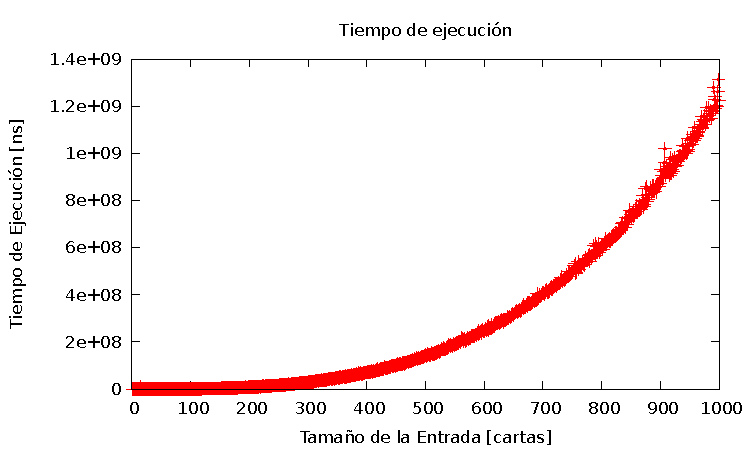
\includegraphics[width=\textwidth]{ej1/cubico.pdf}
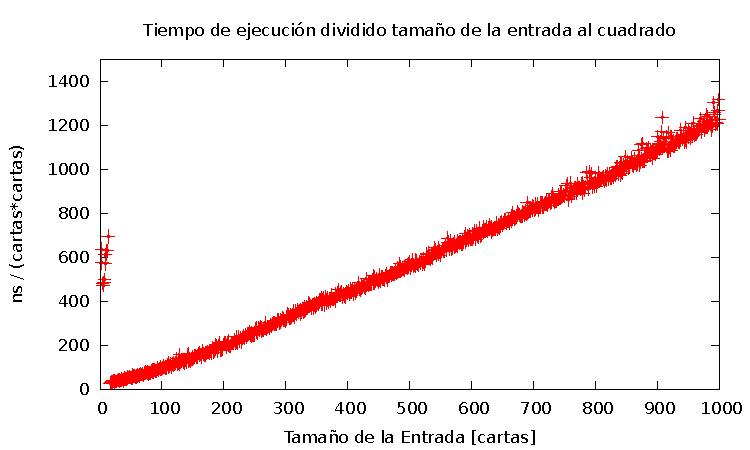
\includegraphics[width=\textwidth]{ej1/lineal.pdf}
%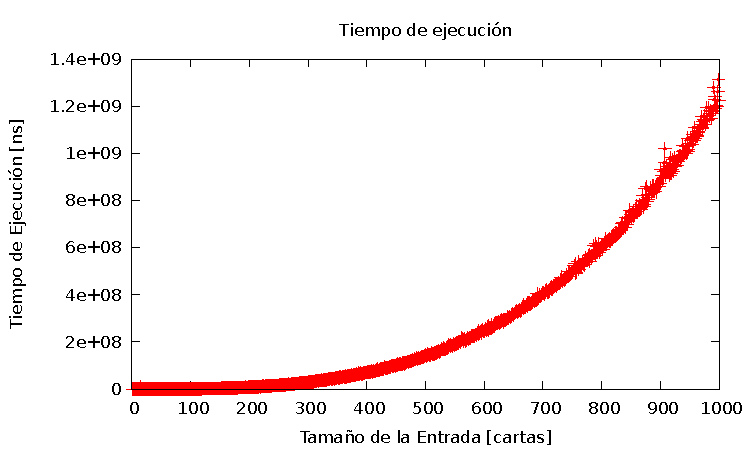
\includegraphics{ej1/cubico.pdf}
%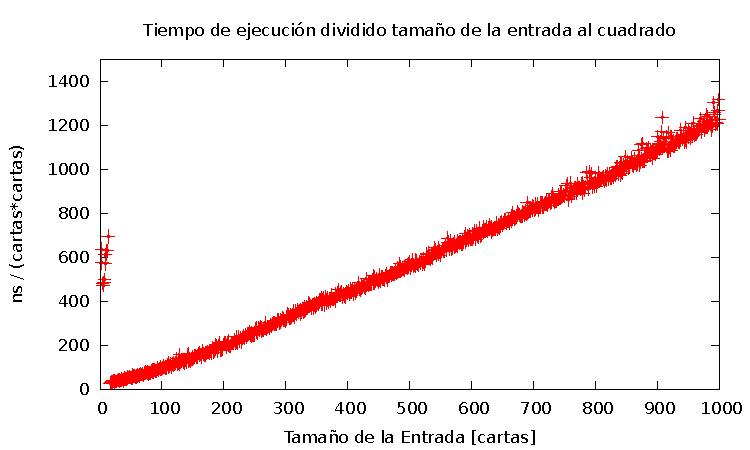
\includegraphics{ej1/lineal.pdf}

\subsection{Compilar y ejecutar}
Desde el directorio src/Ejercicio1:
\begin{itemize}
   \item {\bf Compilar:} ./ej1 make
   \item {\bf Ejecutar:} ./ej1
   \item {\bf Correr casos de test:} ./ej1 tests
   \item {\bf Benchmarks:} ./ej1 bench
\end{itemize}

\subsection{C\'odigo Fuente}
% Cambiar por el que resalta la sintaxis
\begin{verbatim}
public void calcularSolucion() {
 int n = cartas.length;
 for ( int i = 0; i < n; i++ ) {
  cache[i][i] = cartas[i];
  jugadas[i][i].desdeIzquierda( 1 );
 }

 for ( int columna = 1; columna < n; columna++ ) {
  for ( int diagonal = 0; diagonal < n - columna; diagonal++ ) {
   int i = diagonal;
   int j = columna + diagonal;
   int min_ij = Integer.MAX_VALUE;
   int puntos = 0;
   int x = i, y = j;
   for ( int k = i; k <= j; k++ ) {
    int a = 0, b = 0;
    puntos += cartas[k];
    if ( k + 1 <= j ) a = cache[k + 1][j];
    if ( k - 1 >= i ) b = cache[i][k - 1];
    if ( min_ij < a && min_ij < b ) continue;
    if ( a < b ) {
     jugadas[i][j].desdeIzquierda( k - i + 1 );
     min_ij = a;
    } else {
     jugadas[i][j].desdeDerecha( j - k + 1 );
     min_ij = b;
    }
   }
   cache[i][j] = puntos - min_ij;
  }
 }
}
\end{verbatim}
